\section{Decentralization/Distribution: What Sets Them Apart?}

Let us now restate the difference of the concepts of decentralization and distribution in the context of blockchain.

\begin{outline}
\textbf{Decentralization} refers to the distribution of control and decision-making power from a central authority. In blockchain, this means that no single entity has control over the network. Instead, the network is managed by a group of nodes that work together to maintain the integrity of the network.

\textbf{Distribution}, on the other hand, refers to the physical dispersion of data or computing resources in a network. In blockchain, this means that the data and computing resources needed to maintain the network are distributed across multiple nodes. This distribution makes blockchain technology extremely resilient and secure: even if one or more nodes go offline, the network can continue to function because the other nodes can assume their responsibilities.
\end{outline}


\section{Methods of Decentralization}
In this section, we will explore the three distinct degrees of decentralization and how they vary based on the implementation of two key concepts: \textbf{disintermediation} and \textbf{competition-driven decentralization}. 

\begin{enumerate}
\item \textbf{\textcolor{Blue}{Fully Centralized}}: In this case, all operations, controls and decisions are managed by a single central authority or entity. There is no form of decentralization. Disintermediation is absent and there is no competition for control of the network.

\item \textbf{\textcolor{Blue}{Semi-Decentralized}}: In a semi-decentralized structure, some aspects of the system are decentralized, while others are still centrally controlled. This may result in some degree of disintermediation, where some functions can be performed without third-party intervention, but is not completely eliminated. Competition-driven decentralization may be present in some parts of the system, but may not be applied in all aspects.

\item \textbf{\textcolor{Blue}{Fully Decentralized}}: In a fully decentralized system, there is no central authority controlling the system or making decisions. All operations are handled by network users in a distributed manner. This level of decentralization leads to strong disintermediation, where transactions and operations can take place directly between parties without intermediaries. In addition, competition for control of the network can be a key element, where network actors openly compete to influence consensus decisions.
\end{enumerate}

It is clear from the above explanations that decentralization and distribution are two crucial concepts in the design of blockchain networks. However, it is worth noting the \textit{subtle difference} between the two.

Decentralization deals with decision making and who has the power to make decisions (\textbf{governance}), while distribution deals with the physical arrangement of resources in the network (\textbf{technical concept}).

Interestingly, a network can be decentralized without being distributed, and vice versa. However, in practice, most decentralized networks are also distributed (this is because distribution is crucial to ensure network integrity and resilience).

\section{Unveiling the Core of Blockchain}
Finally, we reach the \textit{juiciest part}: the fundamental concepts of blockchain. Let's explore the pillars on which this revolutionary technology is based!

\textbf{\textcolor{Orange}{Nodes}}: Nodes constitute the cornerstone elements of the Blockchain community. They represent the participants or entities that drive the network. These can be computers, laptops or servers belonging to individuals or organizations. Each node assumes a crucial role in the blockchain architecture, contributing its resources and capabilities to the functioning of the entire system.

\textbf{\textcolor{Orange}{Transactions}}: Each transaction in the blockchain represents a major event permanently recorded in digital history. When two or more nodes interact, a transaction is noted in the blockchain through a process known as hashing. This process ensures the security and immutability of each transaction, preserving the integrity of the data transmitted.

\textbf{\textcolor{Orange}{Blockchain}}: Let us now imagine all these transactions organized and collected into blocks. Each block constitutes a key point in the blockchain's history, containing a series of related transactions. These blocks are linked consistently through consensus mechanisms, forming an unbroken chain of information.

\textbf{\textcolor{Orange}{Ledger}}: Finally, there is the ledger, the core of the blockchain. This distributed public ledger is hosted on all community nodes, representing the cornerstone of transparency and authenticity. Every block of transactions finds its place within this ledger, recorded sequentially and accessible to all participants. It is the trusted guardian of every movement and transaction within the blockchain.

\begin{figure}[hb]
\centering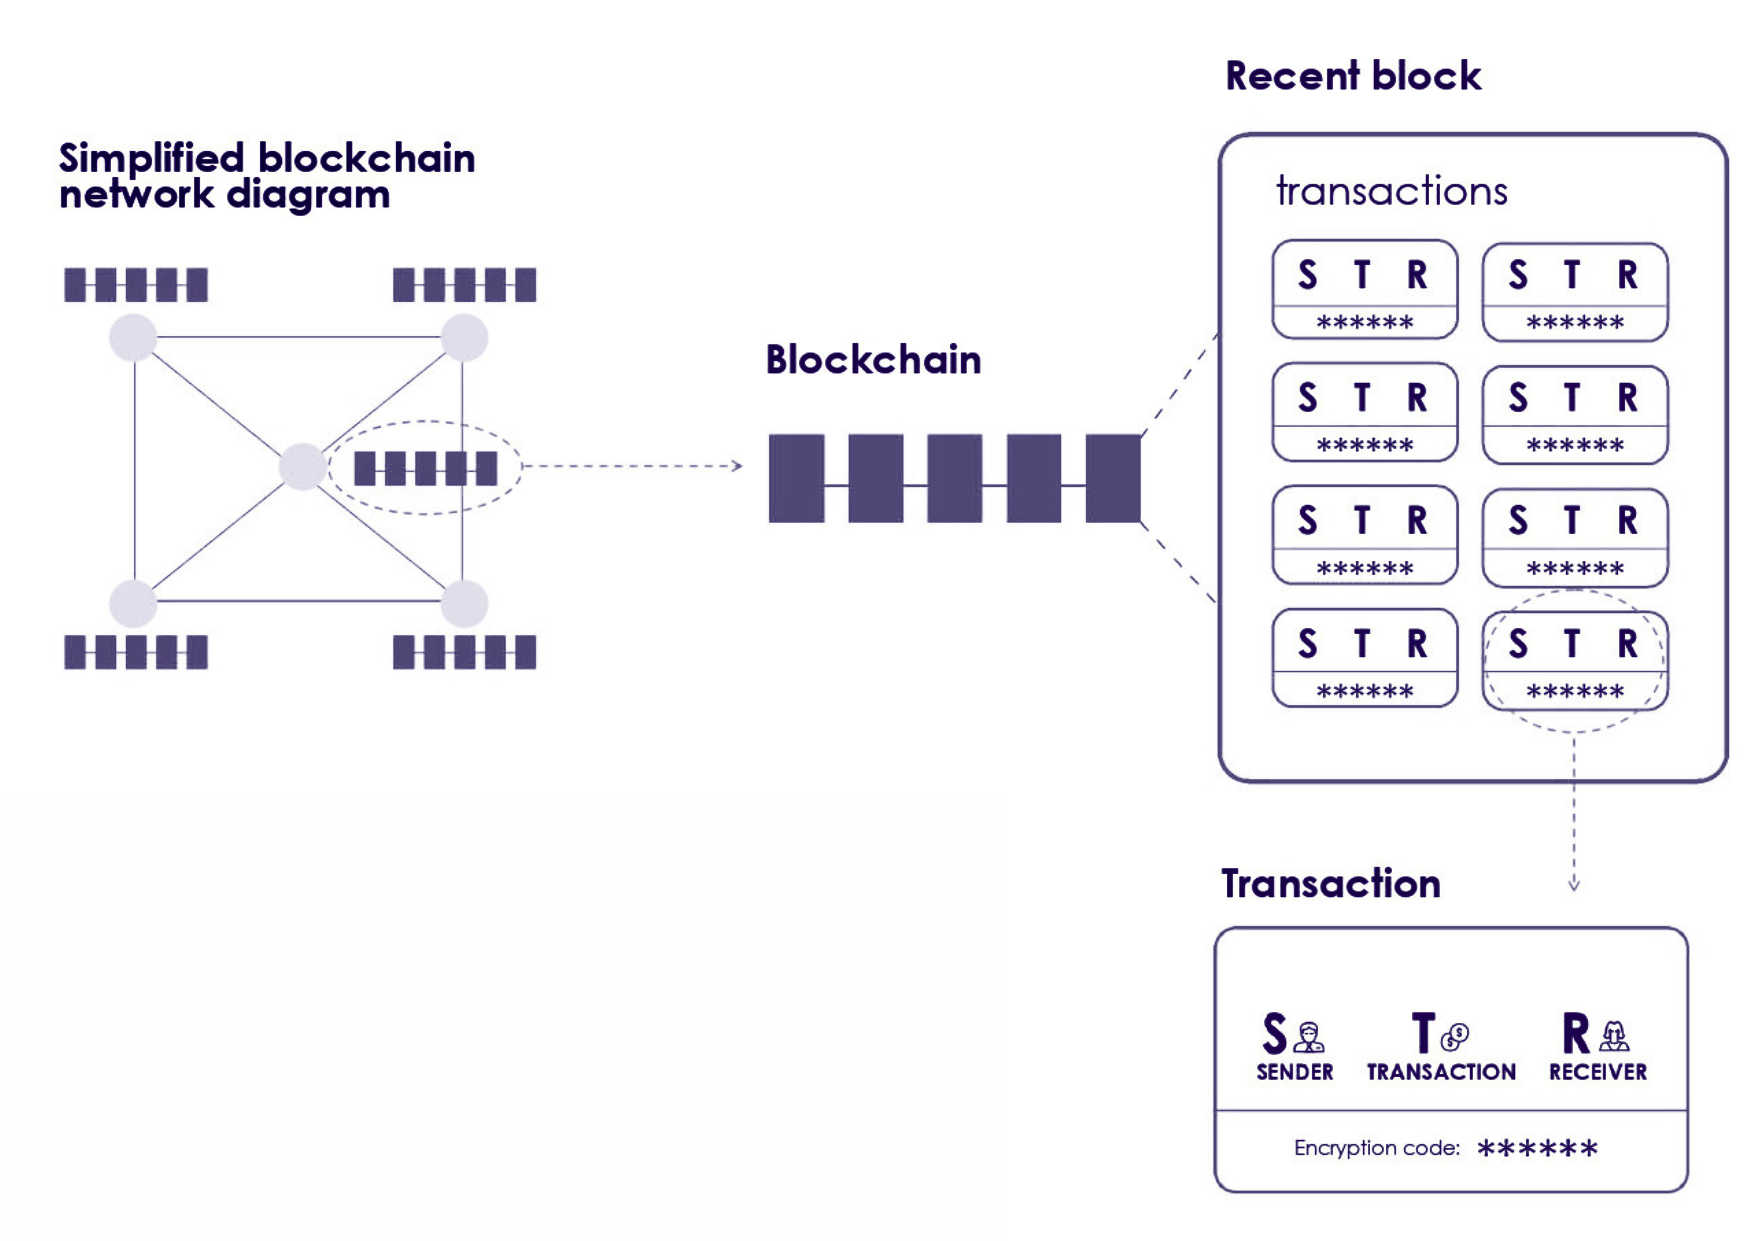
\includegraphics[scale=0.3]{tikz/chapter2 - Blockchain.png}
\caption{Visual Example of the Blockchain \cite{blockchainFinyear}}
\end{figure}


\section{The Anatomy of a Block}

Let's go a little deeper! Let us now examine a block with a magnifying lens  \faSearch

\textbf{\textcolor{Blue}{Header}}:
\begin{itemize}
    \item \textbf{Hash of the Previous Header Link}: This field contains the hash value of the previous block, thus creating an immutable chain of blocks. Hashes, such as the popular SHA-256 (256-bit Secure Hash Algorithm), are cryptographic functions that transform data into fixed-length strings, which are essential for verifying data integrity.
    \item \textbf{Nonce}: This is an arbitrary value that is changed during the mining process until a hash is found that meets specific criteria.
    \item \textbf{Timestamp}: This indicates the precise time when the block was created.
    \item \textbf{Merkle Root}: This is the root hash of a Merkle tree, a data structure that enables efficient verification of the integrity of transactions contained in the block.
\end{itemize}


\textbf{\textcolor{Blue}{Body}}:
\begin{itemize}
    \item \textbf{List of Transactions}: This section lists all the transactions included in the block. Each transaction represents an exchange of value or data within the blockchain network, contributing to the traceability and security of transactions.
\end{itemize}

% \vspace{1cm}
\begin{figure}[hb]
\centering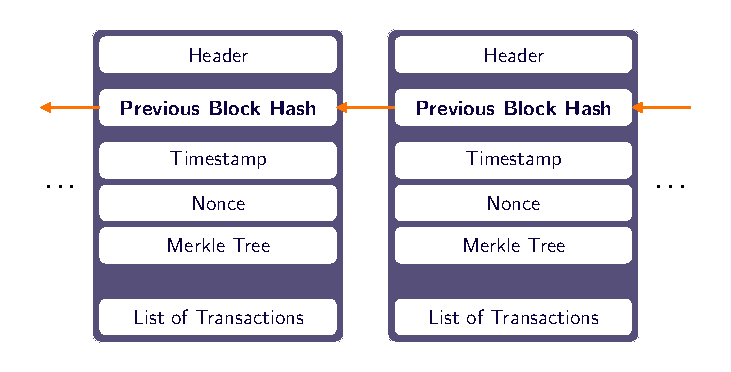
\includegraphics[scale=1.2]{tikz/chapter2 - Blocks.pdf}
\caption{Visual Example of the Blocks}
\end{figure}
